\documentclass{article}
\usepackage[left=0.75in,top=0.6in,right=0.75in,bottom=0.6in]{geometry} %
\usepackage{graphicx}
\begin{document}
	\begin{center}
		%Name,Address,Contact information (Contact,e-mail), Photograph
		\vspace{10px}
	\textbf{\Huge AYUSH LASOD}
	\vspace{10px}
   \line(3,0){500} \\

~\textbullet~ \textbf{\normalsize PES Institute of Technology, Bengaluru-85} ~\textbullet~ {\textbf{\normalsize ayushlasod@gmail.com}} ~\textbullet~ \textbf{\normalsize 9462243355 }
    \vspace{5px}
    
    
\begin{figure}[h]
	\hspace{200pt}
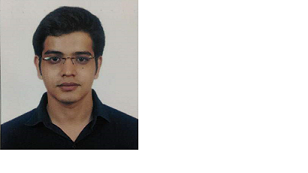
\includegraphics{pic.jpg}
\end{figure}

	%OBJECTIVE

\textbf{\LARGE OBJECTIVE}\\\vspace{10px}
{\large To become associated with a company where I can utilize my skills and gain experience while enhancing the company's productivity
	and reputation.}\\\vspace{15px}

	%EDUCATION

\textbf{\LARGE EDUCATION}\vspace{10px}
\begin{tabular}{|c|c|c|c|c|}\hline
	DEGREE & COLLEGE/SCHOOL & UNIVERSITY & PASSING YEAR & PERCENTAGE \\ \hline
	10th & St. Anselm’s Sr. Sec. School, Bhilwara & CBSE & 2011 & 87.4 \\ \hline
	12th & As' Steward Morris Sr. Sec. School, Bhilwara & CBSE & 2013 & 83.4 \\ \hline
	B.E. (Mech) & PES Institute of Technology, Bengaluru-85 & VTU & 2017 & 74.2 \\ \hline
\end{tabular}\vspace{15px}

	%PROJECTS

\textbf{\LARGE PROJECTS}
\begin{enumerate}
	
	{\large \item •	Final Year Project : Design and Fabrication of Glass Wall Cleaning Robot.\\
		-Presented this Robot Model at e-Yantra Ideas Competition.}
\end{enumerate}\vspace{15px}

	%TRAINING AND INTERNSHIP

\textbf{\LARGE TRAINING AND INTERNSHIP}
\begin{itemize}
	{\large \item \textbf{SANSERA Engineering Pvt. Ltd, Bangalore.}\\
		Studied the process plans of all the automobile
		components like connecting rod, rocker arms, gear shifter
		forks.}
\end{itemize}\vspace{15px}

	% RESEARCH PUBLICATIONS

\textbf{\LARGE RESEARCH PUBLICATIONS}\\NA\vspace{15px}

	%TECHNICAL SKILLS

\textbf{\LARGE TECHNICAL SKILLS}
\begin{itemize}
	{\large \item CAD Software : Solid Edge}
	{\large \item Programming language : Basic C}
	{\large \item MATLAB }
	{\large \item MS-office (Word, PowerPoint, Excel)}
\end{itemize}\vspace{15px}

%SOFT SKILLS

\textbf{\LARGE SOFT SKILLS}
\begin{enumerate}
	{\large \item Leadership}
	{\large \item Teamwork and collaboration }
	{\large \item  Negotiation and Conflict Resolution}
	{\large \item Communication }
	{\large \item Ability to Work Under Pressure }
\end{enumerate}\vspace{15px}

% EXTRA-CURRICULAR ACTIVITIES

\textbf{\LARGE EXTRA-CURRICULAR ACTIVITIES}
\begin{itemize}
	{\large \item AATMATRISHA'16-annual Techno-Cultural fest
		-Core Team Member (headed INFORMAL events) }
	{\large \item AATMATRISHA'15
		-Event Organizer}
	{\large \item SAMARPANA - Support INDIAN ARMY
		-Volunteer }
	{\large \item Quriosa'14 - Annual Science Fest
		-Event Organizer }
\end{itemize}\vspace{15px}

	%CO-CURRICULAR ACTIVITIES

\textbf{\LARGE CO-CURRICULAR ACTIVITIES}
\begin{enumerate}
	{\large \item BOOTSTRAP'15-Practical Skill Development
		Program
		-Instructor for ' ENGINE Breakdown' }
	
	{\large \item •	Industrial visit to Toyota Kirloskar Motor for understanding Lean Manufacturing. }
	{\large \item Runners Up in 'Junkyard Wars',
		An event in Epsilon 2k16, Annual Science fest }
\end{enumerate}\vspace{15px}

\end{center}

%Personal Details

\textbf{\LARGE Personal Details}\\
{\normalsize Father's Name:Munna Lal Lasod\\
	Mother's Name:Nirmala Lasod\\
	Sex:Male\\
	Date of Birth:20th August,1995\\
	Nationality:Indian\\
	Marital Status:Unmarried\\}

	%Reference

\textbf{\LARGE Reference}\\
{\normalsize Dr. D  Sethuram\\
	Professor, Department of Mechanical Engineering\\
	PES University, Bengaluru-85\\
	9448493609, sethuramd@pes.edu\\
	Teacher\\}



\end{document}